
\chapter{Finestra principale}

Sulla destra della tab principale sono presenti 4 tab per leggere le varie risorse Modbus 
"FC 01 Coils", "FC02 Discrete Inputs", "FC 03 Holding Registers" e "FC04 Input Registers".

\section{FC01 - Coils}

La scheda Coils permette di leggere e scrivere uscite digitali con le funzioni FC01/FC05/FC15. I
pulsanti Read/Loop/Write vengono sbloccati solo se la connessione a un dispositivo è andata a
buon fine.

\begin{figure}[H]
\centering
\includegraphics[width=0.85\textwidth]{../Img/Modbus_Client_Coils_00.PNG}
\caption{FC01 - Coils}
\end{figure}

La funzione loop permette di leggere i registri indicati in polling, l'intervallo di interrogazione si
configura nella scheda impostazioni ("Settings"). 
Di default le celle lette vengono colorate di azzurro se il contenuto è popolato (inteso come $>$ 0).
In alto a destra sono presenti i comandi per leggere le risorse di un gruppo o tutte le risorse
di tipo coils configurate nel rpofilo corrente. La configurazione delle risorse così come la creazione e 
associazione dei gruppi viene descritto nel capitolo \ref{template}.

\newpage

Con il box "Read Coil Range" è possibile leggere un range di uscite digitali definito dall'utente,
sarà poi il programma eventualmente a dividere il comando in più richieste FC01 ciascuna di n coils
indicati sopra (nell'esempio seguente pari a 20). 
E' possibile inoltre forzare coils multiple (FC15) utilizzando il form in basso 
("Force Multiple Coils") o importando un file csv precedentemente esportato.

Le coils settate a 1 vengono colorate di verde se la scrittura va a
buon fine:

\begin{figure}[H]
\centering
\includegraphics[width=0.85\textwidth]{../Img/Modbus_Client_Coils_Write_00.PNG}
\caption{FC05 - Write Coils}
\end{figure}

Abilitando la modalità "Live Edit" è possibile modificare direttamente 
le coils editando la colonna "Value", in questo caso quando si modifica la riga il 
programma invia automaticamente il comando FC05 per impostare la coil al valore inserito.

\newpage
\section{FC02 - Discrete inputs}

La scheda Inputs permette di leggere ingressi digitali con le funzioni FC02. I pulsanti Read/Loop
come per la tab Coils vengono sbloccati solo se la connessione a un dispositivo è andata a buon
fine. I pulsanti "Read group" e "Read all" permettono di leggere registri precedentemente configurati 
nel template personalizzato (i registri vengono letti singolarmente sia che siano o meno consecutivi
tra di loro).

\begin{figure}[H]
\centering
\includegraphics[width=0.85\textwidth]{../Img/Modbus_Client_Inputs_00.PNG}
\caption{FC02 - Discrete Inputs}
\end{figure}

Con il box "Read Input Range" è possibile leggere un range di ingressi digitali definito dall'utente,
sarà poi il programma eventualmente a dividere il comando in più richieste FC02
ciascuna di n ingressi specificati nel box delle letture singole (nell'immagine sopra pari a 120).

\newpage
\section{FC03 - Holding registers}

La scheda Holding Registers permette di leggere e scrivere registri digitali a 16 bit con le funzioni
FC03/FC06/FC16.

\begin{figure}[H]
\centering
\includegraphics[width=0.85\textwidth]{../Img/Modbus_Client_HoldingReg_00.PNG}
\caption{FC03 - Holding Registers}
\end{figure}

Il valore del campo "Value" può essere visualizzato sia in decimale (DEC) che in esadecimale
(HEX). Nella tabella è possibile abilitare anche la visualizzazione del corrispondente valore in binario.
Ampliando la finestra è possibile visualizzare informazioni aggiuntive (che vengono configurate
nella finestra template), ad un registro holding infatti è possibile
associare un'etichetta per identificarne il contenuto o visualizzare il valore convertito in integer/
float/string/etc.. Utilizzare il menu a tendina view per configurare le colonne che si desidera visualizzare
nella tabella come mostrato nell'immagine seguente.

\begin{figure}[H]
\centering
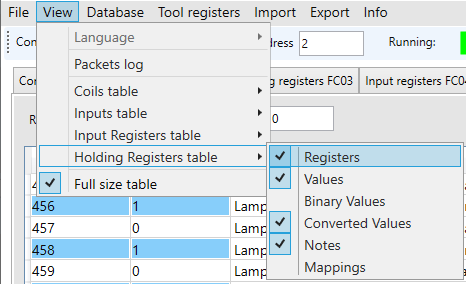
\includegraphics[width=0.40\textwidth]{../Img/Menu_View_Holding.PNG}
\caption{FC03 - View Tab Holding Registers}
\end{figure}

Con il box "Read Holding Register Range" è possibile leggere un range di registri definito
dall'utente (anche > 123), sarà poi il programma eventualmente a dividere il comando in più
richieste FC03 di n registri specificati nel box sopra (nell'immagine 120)
e a popolare la tabella con tutti i registri richiesti.

Spuntando il flag "Live Edit" è possibile inviare la scrittura dei registri automaticamente
modificando una cella delle colonne "Value", "Binary Value" o "Converted Value". La funzione
live risulta molto utile per modificare in diretta i registri visualizzati.

\begin{figure}[H]
\centering

\includegraphics[width=0.40\textwidth]{../Img/ModBus_Client_HoldingReg_Live.PNG}
\caption{FC03 - Live edit}
\end{figure}

Le modifiche alle celle della colonna "Value" vengono inviate con la funzione FC06
(write single register), le modifiche alla colonna "Binary Value" vengono convertite da
binario e inviate sempre come FC06, mentre le modifiche alla colonna "Converted Value"
vengono inviate come FC06 o FC16 a seconda della tipologia del dato configurato (la funzione 
FC16 viene utilizzata
per variabili integer o float a 32 o 64 bit). Nella colonna value è possibile inserire 
valori in esadecimale, se la visualizzazione è già in esadecimale il valore inserito sarà considerato
sempre esadecimale, mentre nella visualizzazione decimale anteporre un "0x"/"x" o postporre un "h"
per indicare che il valore che si vuole inviare è scritto in esadecimale.

La tabella visualizzata può essere esportata in formato .csv o .json con il pulsante "Export" in basso
a destra. Tabelle esportate in csv possono essere importate e inviate allo slave con il pulsante "Import".
Questa funzione risulta comoda quando si vuole copiare una mappa di memoria da un PLC ad un altro o semplicemente
esportare un backup ripristinabile in qualsiasi momento.

\begin{figure}[H]
\centering
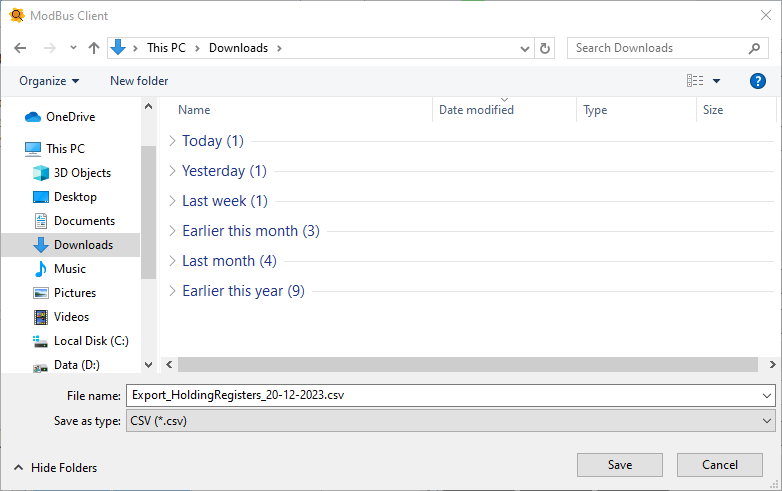
\includegraphics[width=0.70\textwidth]{../Img/ModBus_Client_HoldingReg_Import.PNG}
\caption{FC03 - Form import csv}
\end{figure}

\newpage
\section{FC04 - Input registers}

La scheda Input Registers permette di leggere registri a 16 bit con le funzioni FC04. I pulsanti
Read/Loop come per le altre tab vengono sbloccati solo se la connessione a un dispositivo è
andata a buon fine.

\begin{figure}[H]
\centering
\includegraphics[width=0.85\textwidth]{../Img/Modbus_Client_InputReg_00.PNG}
\caption{FC04 - Input Registers}
\end{figure}

Il valore del campo "Value" può essere visualizzato sia in decimale (DEC) che in esadecimale
(HEX). A fianco viene mostrato anche il valore in binario. Ampliando la finestra è possibile
visualizzare informazioni aggiuntive (che vengono configurate nella finestra template). Ad un
registro infatti è possibile associare un'etichetta per identificarne il contenuto o visualizzare il valore
convertito in integer/float/string/etc.. Per meglio chiarire questa parte si veda la sezione Template.
Con il box "Read Input Register Range" è possibile leggere un range di registri definito dall'utente
(anche > 123), sarà poi il programma eventualmente a dividere il comando in più richieste FC04 e
a popolare la tabella con tutti i registri richiesti.

\begin{figure}[H]
\centering
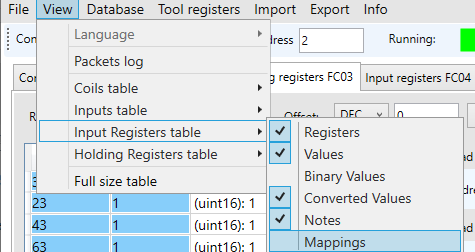
\includegraphics[width=0.60\textwidth]{../Img/Menu_View_InputReg.PNG}
\caption{FC04 - View TabInput Registers}
\end{figure}

Come per gli holding register è possibile selezionare dal menu view quali colonne mostrare nella tabella.

\newpage
\section{Diagnostica}

Nella tab diagnostica è possibile inviare comandi di diagnostica al dispositivo interrogato, 
si presti attenzione
che non tutti i dispositivi rispondono alla funzione FC08.

\begin{figure}[H]
\centering
\includegraphics[width=0.85\textwidth]{../Img/Modbus_Client_Diagnostic_00.PNG}
\caption{FC08 - Diagnostic}
\end{figure}

Funzioni FC08 supportate:

\begin{verbatim}
    - 00 Return Query Data
    - 01 Restart Comunications Option
    - 02 Return Diagnostic Register
    - 03 Change ASCII Input Delimeter
    - 04 Force Listen Only Mode
    - 10 Clear Counters and Diagnostic Register
    - 11 Return Bus Message Count
    - 12 Return Bus Comunication Error Count
    - 13 Return Bus Exception Error Count
    - 14 Return Slave Message Count
    - 15 Return Slave No Response Count
    - 16 Return Slave NAK Count
    - 17 Return Slave Busy Count
    - 20 Clear Overrun Counter and Flag
\end{verbatim}

Nella tab diagnostica inoltre è possibile comporre trame ModBus manualmente, 
nel caso di trame RTU utilizzare il pulsante "Calc CRC" per calcolare e aggiungere in coda al
pacchetto il CRC 16 ModBus.
A livello di protocollo, nella versione RTU vengono aggiunti due byte di CRC
utilizzati dallo slave per verificare l'integrità del pacchetto.
In basso vengono mostrati due esempi di trame ModBus, 
utilizare i due pulsanti per copiare gli esempi nel box della trama.